% !TEX encoding = UTF-8 Unicode

\documentclass[margin=3cm,innermargin=3cm, a0paper, landscape]{tikzposter}
\usepackage{iwona} % body font
\usepackage{eulervm} % set math font
\usepackage[utf8]{inputenc}
\usepackage[T1]{fontenc}
\usepackage{csquotes}
\usepackage{IEEEtrantools}
\usepackage{float,physics,amssymb,amsmath,amsfonts,multicol,dsfont,mathrsfs,cancel,tensor,slashed,mathtools}
\usepackage{bm}
\usepackage{adjustbox}
\usepackage{enumitem}
\usepackage[backend=biber,style=numeric]{biblatex}
\usepackage{poster-theme}
\usepackage{graphicx,caption,tikz,xparse,subcaption}
\usetikzlibrary{arrows.meta}
\usepackage{svg} % for svg images directly from inkscape e.g.
\usepackage{mwe} % for placeholder images

\usepackage[compat=1.1.0]{tikz-feynman}

\graphicspath{{images/}}

\addbibresource{ref.bib}

% set theme parameters
\tikzposterlatexaffectionproofoff
\usepackage{anyfontsize}
\usetheme{MyTheme}
\usecolorstyle{MyStyle}

\title{\parbox{\linewidth}{\centering Big important title}}
\author{Foo Foo$^{*\dagger}$ and Bar Bar$^{\dagger}$}
\institute{
    \textsuperscript{$\dagger$}Department of Atmospheric and Oceanic Sciences, McGill University, Montr\'eal, Canada\\
    \textsuperscript{$*$}\emph{Corresponding author email:} foo.foo@mail.mcgill.ca 
}

\titlegraphic{
\includegraphics[width=0.15\textwidth]{mcgill_logo.png}}

\begin{document}
\maketitle

\begin{columns}
    
    \column{0.26}
    
        \block{{\fontsize{50}{60}\selectfont Context title}}
        {
            % petites figures
            \begin{tikzpicture}[remember picture,overlay]
                \node[xshift=19cm,yshift=-4cm,anchor=north west] at (current page.north west){%
                \includegraphics[scale=1.1]{example-image-b}}; % your face
                \node[xshift=6cm,yshift=-4cm,anchor=north west] at (current page.north west){%
                \includegraphics[scale=1.1]{example-image-a}}; % your QR code
                \node[xshift=19cm,yshift=-18cm,anchor=north west] at (current page.north west){%
                \includesvg[scale=3.3]{arrow.svg}}; % big arrow
                %\node[xshift=8cm,yshift=-14.5cm,anchor=north west] at (current page.north west){%
                %\includesvg[scale=0.14]{fissure.svg}};
            \end{tikzpicture}
            {\fontsize{40}{48}\selectfont 
            \begin{itemize}
            
                \item context 1
                \item context 2
                \item context 3
        
            \end{itemize}
            }
        }
        
        \block{{\fontsize{50}{60}\selectfont Need title}}
        {
            
            % petites figures
            \begin{tikzpicture}[remember picture,overlay]
                %\node[xshift=27cm,yshift=-31cm,anchor=north west] at (current page.north west){%
                %\includesvg[scale=0.25]{radar.svg}};
                %\node[xshift=30cm,yshift=-25cm,anchor=north west] at (current page.north west){%
                %\includesvg[scale=0.5]{qr_ice.svg}};
            \end{tikzpicture}
            {\fontsize{40}{48}\selectfont
            \begin{itemize}
            
                \item task 1
                \item task 2
                \item task 3
        
            \end{itemize}
            \begin{center}
                \begin{minipage}{0.8\linewidth}
                    \begin{figure}[H]
                        \begin{center}
                        
                            \includegraphics[width=\linewidth]{example-image-golden}\\
                            \caption*{\large caption}
                            
                        \end{center}
                    \end{figure}
                \end{minipage}
            \end{center}
            
            \innerblock{{\fontsize{50}{60}\selectfont Object of poster}}
            {
                % petites figures
                \begin{tikzpicture}[remember picture,overlay]
                    %\node[xshift=4.8cm,yshift=-59.6cm,anchor=north west] at (current page.north west){%
                    %\includesvg[scale=0.38]{lightbulb.svg}};
                    \node[xshift=3cm,yshift=-73.5cm,anchor=north west] at (current page.north west){%
                    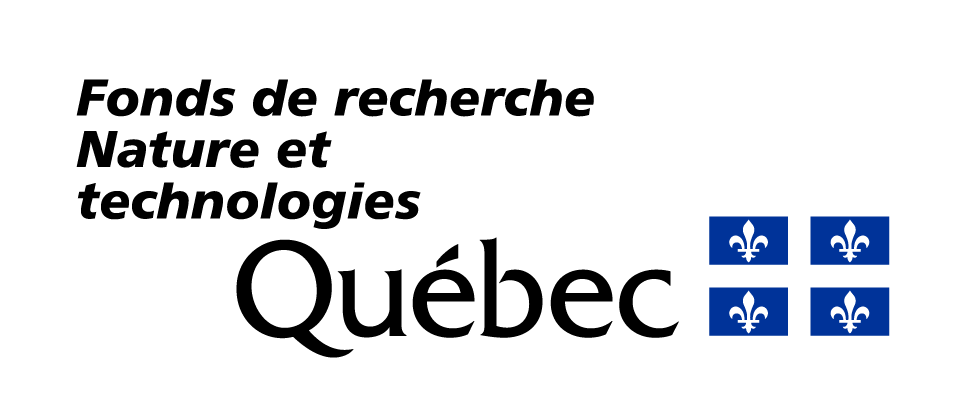
\includegraphics[scale=0.5]{logo-frqnt-couleur.png}};
                    \node[xshift=103cm,yshift=-75cm,anchor=north west] at (current page.north west){%
                    
\includegraphics[scale=0.7]{ArcTrain.png}};
                \end{tikzpicture}
                {\fontsize{40}{48}\selectfont 
                \begin{itemize}
            
                    \item object 1
                    \item object 2 
        
                \end{itemize}
                }
            }
            }
            
        }
    \column{0.12}    % column of free space
    \column{0.50}    % column where the block is
    
        \block{{\fontsize{50}{60}\selectfont How or model}}
        {
            {\fontsize{40}{48}\selectfont 
            
                    \begin{minipage}[c]{\linewidth}
                        \begin{IEEEeqnarray}{rCl}
                            \bar{u}_2(-ie\Gamma^\mu )u_1&=&
                            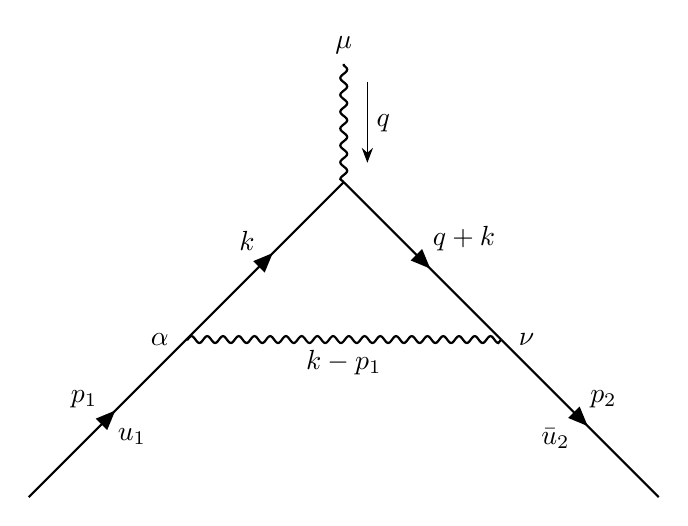
\begin{tikzpicture} [baseline=5ex]
                                \begin{feynman} [large]
                                    \vertex (a1);
                                    \vertex [right=of a1] (b1);
                                    \vertex [right=of b1] (c1);
                                    \vertex [right=of c1] (d1);
                                    \vertex [right=of d1] (e1);
                                    \vertex [above=of c1] (c2);
                                    \vertex [right=of c2] (d2);
                                    \vertex [left=of c2] (b2);
                                    \vertex [above=of c2] (c3);
                                    \vertex [above=1.5cm of c3] (c4) {$\mu$};
                                    \vertex [right=.1cm of d2] (e2) {$\nu$};
                                    \vertex [left=.1cm of b2] (a2) {$\alpha$};
                                    
                                    \diagram* 
                                    {
                                    {[edge={fermion}]
                                    (a1) -- [edge label=$p_1$, edge label'=$u_1$] (b2),
                                    (b2) -- [edge label=$k$] (c3),
                                    (c3) -- [edge label=$q+k$] (d2),
                                    (d2) -- [edge label=$p_2$, edge label'=$\bar{u}_2$] (e1),
                                    },
                                    {[edge={photon}]
                                    (b2) -- [edge label'=$k-p_1$] (d2),
                                    (c4) -- [momentum=$q$] (c3),
                                    },
                                    }; 
                                \end{feynman}
                            \end{tikzpicture}
                            +\mathcal{O}(e^5)\nonumber\\
                            &=&(-ie)^3\int\frac{\dd^4k}{(2\pi)^4}\frac{-ig_{\alpha\nu}}{(k-p_1)^2}\bar{u}_2\gamma^\nu\frac{i(\slashed{q}+\slashed{k}+m)}{(q+k)^2-m^2}\gamma^\mu\frac{i(\slashed{k}+m)}{k^2-m^2}\gamma^\alpha u_1\nonumber.
                        \end{IEEEeqnarray}
                    \end{minipage}
            }
        }
    
    % oh you could also split it even further!
    \begin{columns}
    
        \column{0.26} % first column
        
        \column{0.37} % column result 1
    
            \block{{\fontsize{50}{60}\selectfont Results 1 title}}
            {   
                 % petites figures
                \begin{tikzpicture}[remember picture,overlay]
                    %\node[xshift=91cm,yshift=-16.5cm,anchor=north west] at (current page.north west){%
                    %\includesvg[scale=0.15]{rouages.svg}};
                \end{tikzpicture}
                {\fontsize{40}{48}\selectfont 
                
                \begin{center}
                    \begin{minipage}{0.8\linewidth}
                        \begin{figure}[H]
                            \begin{center}
                            
                                \includegraphics[scale=5]{example-grid-100x100pt}\\
                                \caption*{\large caption}
                                
                            \end{center}
                        \end{figure}
                    \end{minipage}
                \end{center}
                
                }
            }
    
        \column{0.37} % column result 2
            
            \block{{\fontsize{50}{60}\selectfont Results 2 title}}
            {
                % petites figures
                \begin{tikzpicture}[remember picture,overlay]
                    %\node[xshift=85cm,yshift=-16cm,anchor=north west] at (current page.north west){%
                    %\includesvg[scale=0.2]{console.svg}};
                \end{tikzpicture}
                {\fontsize{40}{48}\selectfont 
                
                \begin{center}
                    \begin{minipage}{0.8\linewidth}
                        \begin{figure}[H]
                            \begin{center}
                            
                                \includegraphics[scale=5]{example-grid-100x100pt}\\
                                \caption*{\large caption}
                                
                            \end{center}
                        \end{figure}
                    \end{minipage}
                \end{center}
                
                }
            }
            
    \end{columns}
    
    \begin{columns}
    
        \column{0.26}
        \column{0.12}
        \column{0.50}
            % you can move it with the offsets here
            \block[bodyoffsety=0cm,titleoffsety=0cm]{{\fontsize{50}{60}\selectfont Take-home message}}
            {
                \innerblock{}{\centering {\fontsize{50}{60}\selectfont Take-home message}}
                
                \begin{tikzpicture}[remember picture,overlay]
                  %  \node[xshift=46.5cm,yshift=-66.5cm,anchor=north west] at (current page.north west){%
                  %  \includesvg[scale=0.4]{file.svg}};
                \end{tikzpicture}
            }
    
    
    
    \end{columns}

\end{columns}


\end{document}